\documentclass[serif, aspectratio=169]{beamer}

\usetheme{metropolis}

% Define title
\newcommand{\doctitle}{MECO4114 Research Methods}
\newcommand{\docsubtitle}{Week 06 Digital Research Methdos}% Remove if not needed

% Define author
\newcommand{\docauthor}{Francesco Bailo}
% \newcommand{\docauthortitle}{PhD Student}
\newcommand{\docauthorinstitute}{The University of Sydney}
\newcommand{\docauthoremail}{francesco.bailo@sydney.edu.au}
\newcommand{\InstitutePlace}{Institue and place}

% Define subject and keywords
\newcommand{\docsubject}{ADD SUBJECT HERE}
\newcommand{\dockeywords}{Keywords;}

% Define creation date (format D:YYYYMMDDHHmmss)
\newcommand{\doccreationdate}{D:20240326}

%% Bibliography - Start %%

% Set the values for the bibliography
\usepackage[
    style=apa,
    indexing,
    backend=biber,
    isbn=false,
    url=true,
    doi=true,
    eprint=false,
    hyperref=true,
    backref=false,
    firstinits=false,
    natbib  
]{biblatex}

% Recommended by biblatex
\usepackage[utf8]{inputenc}
\usepackage{textcomp}
\usepackage{xpatch}

% Remove series & edition
\AtEveryBibitem{
  \clearfield{series}
  \clearfield{edition}
}

% Remove month and day only for journal article
\AtEveryBibitem{%
  \ifboolexpr{test {\ifentrytype{article}} and (not test {\iffieldundef{number}} or not test {\iffieldundef{volume}})}
    {\clearfield{month}
     \clearfield{day}
     \clearfield{url}
     \clearfield{urldate}}
     {}%
}

% Remove month for books
\AtEveryBibitem{%
  \ifentrytype{book}{%
    \clearfield{month}%
    \clearfield{day}%
  }{%
  }%
}

% Remove url for 
\AtEveryBibitem{%
  \ifentrytype{book}{%
    \clearfield{month}%
    \clearfield{day}%
  }{%
  }%
}

% Suppress urldate and url for all items except misc. In biblatex option url need to be set to true 
% \savebibmacro{url+urldate} \renewbibmacro*{url+urldate}
% {\ifentrytype{misc}{\restorebibmacro{url+urldate}\usebibmacro{url+urldate}}{}}

% Add "reprinted from" at the end of the reference
\renewbibmacro*{related:reprintfrom}[1]{%
  \entrydata*{#1}{%
    \printtext{\mkbibemph{\printfield[apacase]{booktitle}}}%
    \setunit{\bibpagespunct}%
    \printfield{pages}%
    \setunit{\addcomma\addspace}%
    \bibstring{byauthor}\addspace
    \printnames[apanames][-\value{listtotal}]{editor}%
    \ifnameundef{editor}
      {}
      {\addcomma\addspace
       \usebibmacro{apaeditorstrg}{editor}}
    \printnames[apanames][-\value{listtotal}]{author}%
    \setunit{\addcomma\addspace}%
    \usebibmacro{date}%
    \setunit{\addcomma\addspace}%
    \usebibmacro{location+publisher}%
    \newunit\newblock
    \usebibmacro{related}}}

\DefineBibliographyStrings{british}{
  reprintfrom = {Reprinted from}
}

% Remove origin date if reprint
\renewbibmacro*{origyear}{%
  \ifboolexpr{not test {\iffieldundef{labelyear}} and not test {\iffieldsequal{labelyear}{origyear}} and not test {\iffieldequalstr{relatedtype}{reprintfrom}}}
    {\printfield{origyear}}
    {}}

% Set language and quotes
\usepackage{csquotes}
\usepackage[british]{babel}
\DeclareLanguageMapping{british}{british-apa}


%Point to the bibliography db
\addbibresource{bibliography.bib}

%% = Bibliography - End = %%
% To read acronym file
\usepackage[nolist]{acronym}

\setbeamertemplate{sidebar right}{}
\setbeamertemplate{footline}{%
\hfill\usebeamertemplate***{navigation symbols}
\hspace{1cm}\insertframenumber{}/\inserttotalframenumber}

\renewcommand\rmdefault{pplx}
\renewcommand\mathfamilydefault{cmr}
\usepackage{adjustbox}

% Number style
\usepackage[osf,sc]{mathpazo}

% Reference to list items
% \usepackage[loadonly]{enumitem} % <- Incompatible

% Comment out section by \begin{comment} & \end{comment}
\usepackage{comment}

%Reference name instead of number
\usepackage{nameref}

% Figures, letter spacing and caption style
\usepackage{microtype}
\usepackage[font={small,it},labelfont=bf]{caption}
\usepackage[font={scriptsize,it}]{subcaption}
\captionsetup{compatibility=false}
% \usepackage[font={rm,md,up},margin=10pt,singlelinecheck=false]{subfig}
\usepackage{tikz}
\usetikzlibrary{arrows, positioning, shapes.geometric, shadows, backgrounds, decorations.text}
\usepackage{soul}

% Font encoding. Among others, solve problems with accented chars in output
\usepackage[T1]{fontenc}

% Paragraph spacing
\usepackage{parskip}

% For tables
\usepackage{pgfplotstable}
\usepackage{booktabs}
\usepackage{array}
\usepackage{etoolbox} 
\usepackage{dcolumn}

% \newcolumntype{C}{>{\centering\arraybackslash}m{2.5em}}
% \newcolumntype{D}{>{\arraybackslash}m{15em}}
% \newcolumntype{E}{>{\centering\arraybackslash}m{3.4em}}
% \newcolumntype{F}{>{\centering\arraybackslash}m{4.4em}}

\pgfplotstableset{
    %font={\small},
    empty cells with={--}, %  replace empty cells with ’--’
    every head row/.style={before row=\toprule,after row=\midrule},
    every last row/.style={after row=\bottomrule}
}

%Separate digits with comma (e.g. 1,000,000)
\usepackage[group-separator={,}]{siunitx}
\sisetup{
  detect-all,
  detect-inline-family=math,
  detect-inline-weight=math,
  detect-display-math=true,
  round-mode=places,
  round-precision=2,
  round-minimum = 0.01}

\usepackage{amsmath}

% Set up the images/graphics package
\usepackage{graphicx}
\setkeys{Gin}{width=\linewidth,totalheight=\textheight,keepaspectratio}
\graphicspath{{graphics/}}
\newsavebox\mybox % <- To save size of a picture

% After table/figure space with no idennt
\def\changebreak{\par\vspace{\baselineskip}\noindent}

% The units package provides nice, non-stacked fractions and better spacing
% for units.
\usepackage{units}

% The fancyvrb package lets us customize the formatting of verbatim
% environments.  We use a slightly smaller font.
\usepackage{fancyvrb}
\fvset{fontsize=\normalsize}

% Small sections of multiple columns
\usepackage{multicol}

% Provides paragraphs of dummy text
\usepackage{kantlipsum}

% Figure size
\newlength\onecolumnimage
\setlength\onecolumnimage{.45\textwidth}
\newlength\halfcolumnimage
\setlength\halfcolumnimage{.25\textwidth}

% % Adds a bookmark and table-of-contents line as if it were a subsection

% \AtBeginSection{\frame{\tableofcontents[currentsection]}}

% \usepackage{bookmark}
% \usepackage{etoolbox}
% \makeatletter
% % save the current definition of \beamer@@frametitle
% \let\nobookmarkbeamer@@frametitle\beamer@@frametitle
% % then patch it to do the bookmarks and/or TOC entries
% \apptocmd{\beamer@@frametitle}{%
%   % keep this to add the frame title to the TOC at the "subsection level"
%   % \addtocontents{toc}{\protect\beamer@subsectionintoc{\the\c@section}{0}{#1}{\the\c@page}{\the\c@part}%
%   %     {\the\beamer@tocsectionnumber}}%
%   % keep this line to add a bookmark that shows up in the PDF TOC at the subsection level
%   \bookmark[page=\the\c@page,level=3]{#1}%
%   }%
%   {\message{** patching of \string\beamer@@frametitle succeeded **}}%
%   {\errmessage{** patching of \string\beamer@@frametitle failed **}}%

% \pretocmd{\beamer@checknoslide}{%
%   % ensure the bookmark is not created if the slide is filtered out
%   \let\beamer@@frametitle\nobookmarkbeamer@@frametitle
%   }%
%   {\message{** patching of \string\beamer@checknoslide succeeded **}}%
%   {\errmessage{** patching of \string\beamer@checknoslide failed **}}%

%  \makeatother

%Create Hyperlinks
% To be loaded after everything (except: cleveref, amsrefs, float before hyperref before algorithm, chappg, sidecap, linguex)
\usepackage{hyperref}
\hypersetup{
  pdfinfo={
    Title={\doctitle},
    Author={\docauthor},
    Subject={\docsubject},
    Keywords={\dockeywords},
    CreationDate={\doccreationdate},
    Creator={Typeset with LaTeX}
  },
  linktoc=all
  % colorlinks,
  % citecolor=blue,
  % filecolor=blue,
  % linkcolor=blue,
  % urlcolor=blue
}
\usepackage{url}


% Beamer buttons

\setbeamertemplate{button}{\tikz
  \node[
  inner xsep=4pt,
  draw=structure!80,
  fill=structure!50,
  rounded corners=4pt]  {\tiny\insertbuttontext};}

%----------------------------------------------------------------------------------------
%	TITLE SECTION
%----------------------------------------------------------------------------------------

\title{\doctitle} % Article title

\author{
\large
\textsc{Francesco Bailo}\\[2mm] 
\normalsize The University of Sydney \\
% \normalsize \href{mailto:\docauthoremail}{\docauthoremail} 
% \vspace{-5mm}
}

\titlegraphic{
\includegraphics[height=0.5cm]{figure/Usyd_logo.png}}

\date{27 Mar 2024}

\usepackage[titletoc]{appendix}

%----------------------------------------------------------------------------------------


%----------------------------------------------------------------------------------------
%	HEADER AND FOOTER SECTION
%----------------------------------------------------------------------------------------

\setbeamertemplate{headline}{%
\leavevmode%
  \hbox{%
    \begin{beamercolorbox}[wd=\paperwidth,ht=2.5ex,dp=1.125ex]{palette quaternary}%
    \insertsectionnavigationhorizontal{\paperwidth}{}{\hskip0pt plus1filll}
    \end{beamercolorbox}%
  }
}


\setbeamertemplate{footline}[text line]{%
  \parbox{\linewidth}{\vspace*{-8pt}\href{mailto:\docauthoremail}{\docauthoremail}\hfill\insertpagenumber/\insertpresentationendpage
}}

%----------------------------------------------------------------------------------------

\newcommand{\customcite}[1]{\citeauthor{#1}, \citetitle{#1}, \citeyear{#1}}


\usepackage{newverbs}
\newverbcommand{\bverb}
  {\begin{lrbox}{\verbbox}}
  {\end{lrbox}\colorbox{gray!30}{\box\verbbox}}

\begin{document}

{
\setbeamertemplate{headline}{} 
\setbeamertemplate{footline}{} 
\begin{frame}
  \titlepage
\end{frame}
}
\addtocounter{framenumber}{-1}

\frame{\tableofcontents}


\section{Observing behaviour}

\begin{frame}

\begin{columns}
\begin{column}{0.4\textwidth}

This section is largely based on Chapter 2 of \citetitle{salganik_bit_2018} by Matthew Salganik (2018).

\end{column}

\begin{column}{0.6\textwidth}

\begin{figure}

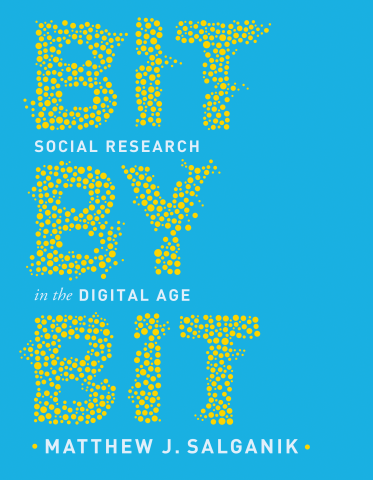
\includegraphics[width=0.7\textwidth]{figure/9780691158648.png}

\end{figure}

\end{column}
\end{columns}

\end{frame}

\begin{frame}

Whatever the subject of your research, there are mainly three ways to collect data: 

\begin{enumerate}

\item<1-> Running experiments

\item<2-> Asking questions

\item<3-> Observing behaviour $\leftarrow$

\end{enumerate}

\begin{itemize}
\item <4-> Observational data are collected without interfering with either
\begin{itemize}
\item<4-> the subject of the investigation or 
\item<4-> the environment of the subject of the investigation.
\end{itemize}
\end{itemize}

\end{frame}

\begin{frame}

\begin{columns}
\begin{column}{0.4\textwidth}

Observation of something or somebody is the primordial way of investigating what we are interested in (and usually the beginning of an investigation). \\~\

Using instruments and sensors to observe and record what we observe is not new.  \\~\

What is new is the number of instruments and sensors that monitor and record human behaviour.


\end{column}
\begin{column}{0.6\textwidth}

\begin{figure}

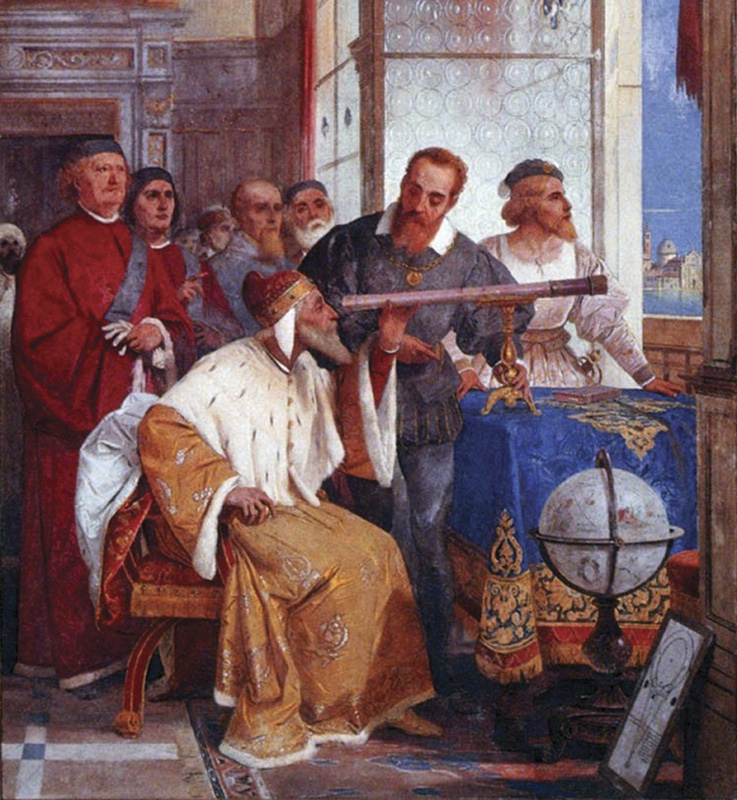
\includegraphics[width=0.7\textwidth]{figure/Bertini_fresco_of_Galileo_Galilei_and_Doge_of_Venice}
\caption{\footnotesize{\citetitle{bertini_galileo_1858}, \cite{bertini_galileo_1858}}}
\end{figure}

\end{column}
\end{columns}

\end{frame}


\begin{frame}

The combination of \textit{flow} and the \textit{stock} of data produced by these instruments and sensors is often called \textbf{Big Data}. 

Big data are \textit{big} on three dimensions: 

\begin{itemize}

\item \textbf{V}olume
\item \textbf{V}ariety
\item \textbf{V}elocity

\end{itemize}

\end{frame}

\begin{frame}

\begin{itemize}

\item<1> So... can you think of any example of big data or source of big data? 

\end{itemize}

\begin{itemize}

\item<2-> Big data are not only data generated by the online activity of users and are not only created by companies. 

\end{itemize}

\begin{enumerate}

\item<3-> Big data are generated online and offline every time a sensor records a human behaviour. 

\item<4-> Big data are created by companies and governments.

\end{enumerate}

\end{frame}


\begin{frame}

\enquote{Big data are created and collected by \textbf{companies} and \textbf{governments} for purposes other than research. Using this data for research therefore requires repurposing.} \autocite[14]{salganik_bit_2018}\\~\ \\~\
\begin{columns}
\begin{column}{0.4\textwidth}
\centering
\includegraphics[width=0.5\textwidth]{figure/300px-Twitter_bird_logo_2012}
\end{column}

\begin{column}{0.2\textwidth}
\LARGE\centering$\neq$
\end{column}

\begin{column}{0.4\textwidth}
\centering
\includegraphics[width=0.7\textwidth]{figure/640px-ABS_Census_Logo}
\end{column}

\end{columns}

\end{frame}

\begin{frame}

According to \autocite{salganik_bit_2018}, Big Data shares ten characteristics. 

\begin{enumerate}

\item<1-> Big Data are \textbf{big}: Rare events, heterogeneity, small differences. \textit{But} how data were created?

\item<2-> Big Data are \textbf{always-on}: Unexpected events and real-time estimates. \textit{But} the systems that collected the data are constantly changing (see \textit{drifting} later)!

\item<3-> Big Data are \textbf{nonreactive}: Measurement is less likely to change behaviour. \textit{But} a social desirability bias persists. 

\item<4-> Big Data are \textbf{incomplete}: No demographic information, no information on behaviour on other platforms, and no data to operationalise theoretical constructs (e.g. \enquote{intelligence}).

\item<5-> Big Data are \textbf{inaccessible}: Access is controlled and conditional. 

\end{enumerate}

\end{frame}

\begin{frame} 

\begin{enumerate}

\setcounter{enumi}{5}

\item<1-> Big Data are \textbf{non-representative}: Data do not come from a probabilistic random population sample. 

\item<2-> Big Data are \textbf{drifting}: Population drift, behavioural drift, system drift. Systems keep changing all the time!

\item<3-> Big Data are \textbf{algorithmically confounded}: Engineering choices impact user behaviours. Also, performativity issues.

\item<4-> Big Data are \textbf{dirty}: Dirty data can be created unintentionally or intentionally (e.g. bots). 

 \item<5-> Big Data are \textbf{sensitive}: The potential sensitivity of the data is always difficult to assess. 

\end{enumerate}

\end{frame}

\section{Network analysis}

\subsection{A very short introduction}

\begin{frame}

\begin{block}{Relations, not attributes. Networks, not groups.}
[S]ocial network analysts argue that causation is not located in the individual, but in the social structure. While people with similar attributes may behave similarly, explaining these similarities by pointing to common attributes misses the reality that \textit{individuals with common attributes often occupy similar positions in the social structure}. That is, \textit{people with similar attributes frequently have similar social network positions}. Their similar outcomes are caused by the \textbf{constraints}, \textbf{opportunities} and \textbf{perceptions} created by these similar network positions. \autocite[13]{marin_social_2011}
\end{block}

\end{frame}

\begin{frame}

\begin{columns}
\begin{column}{0.6\textwidth}
\begin{figure}
    \centering
    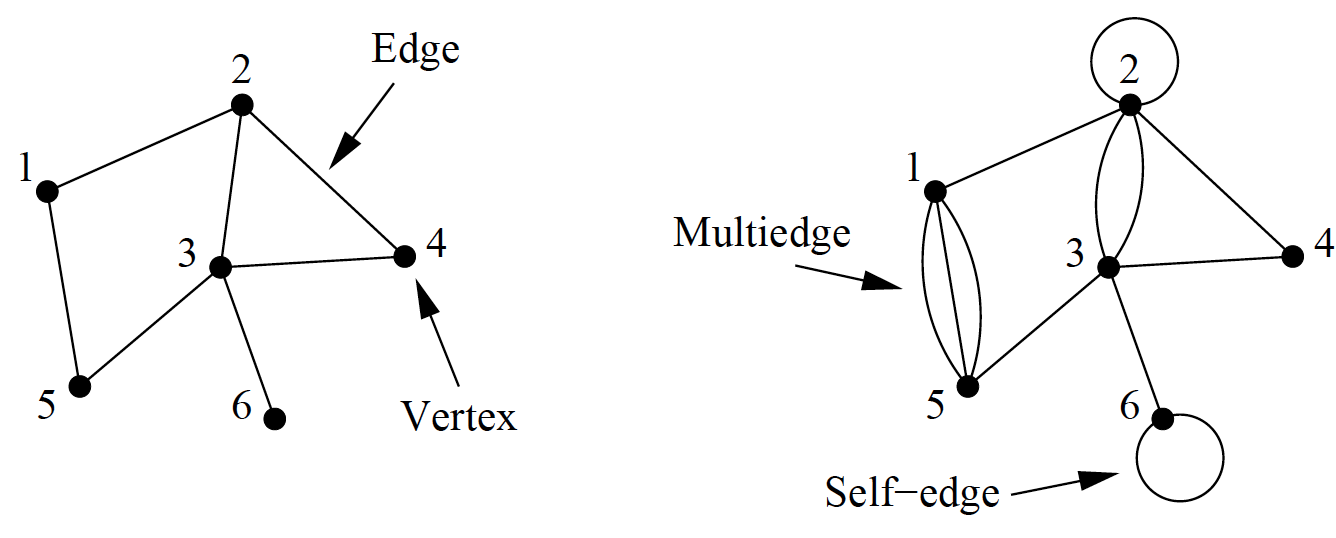
\includegraphics{figure/undirected_network}
\caption{Traditional visualisation of two small networks...}
\end{figure}
\end{column}
\begin{column}{0.4\textwidth}
\begin{figure}
    \centering
    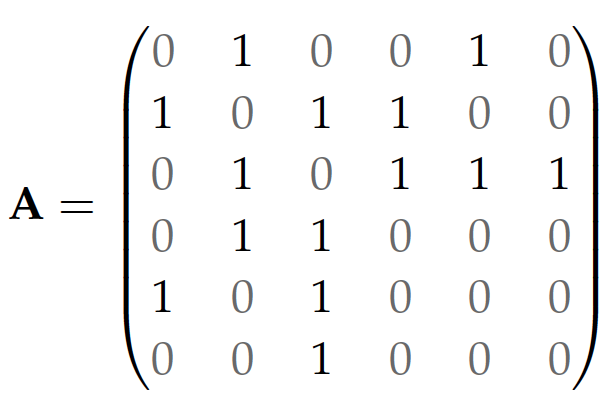
\includegraphics{figure/undirected_adj_matrix}
\caption{... and the adjacency matrix of the left-hand network \autocite[111]{newman_networks_2010}.}
\end{figure}
\end{column}
\end{columns}
\end{frame}

\begin{frame}

\begin{columns}
\begin{column}{0.5\textwidth}
\begin{figure}
    \centering
    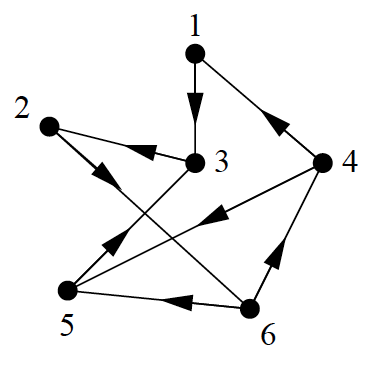
\includegraphics[width = 0.7\textwidth]{figure/directed_network}
\caption{A directed network...}
\end{figure}
\end{column}
\begin{column}{0.5\textwidth}
\begin{figure}
    \centering
    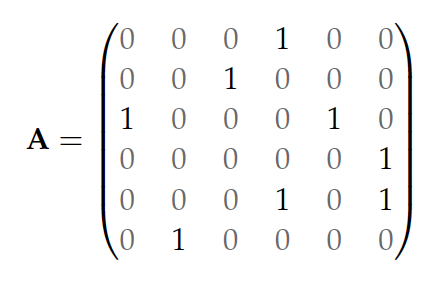
\includegraphics{figure/directed_adj_matrix}
\caption{... and its adjacency matrix (not symmetric!) \autocite[112]{newman_networks_2010}.}
\end{figure}
\end{column}
\end{columns}
\end{frame}

\begin{frame}
{Network measures}

\begin{columns}
\begin{column}{0.6\textwidth}
  \begin{description}
  \item<1-> [Degree of a vertex] number of connections
  \item<2-> [Authority of a vertex] number of important connections
  \item<3-> [Closeness of a vertex] mean distance to other vertices
  \item<4-> [Betweenness of a vertex] extent to which a vertex lies on paths between other vertices
  \item<5-> [Group of vertices]
  \end{description}
\end{column}
\begin{column}{0.4\textwidth}
\begin{figure}
    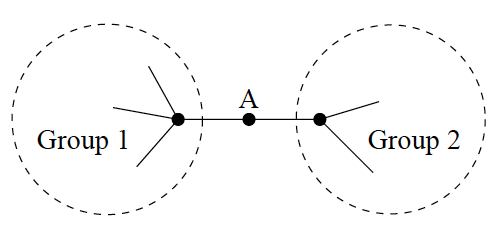
\includegraphics[width=0.55\linewidth]{figure/betweenness}
\end{figure}
\begin{figure}\vspace{.5 cm}
    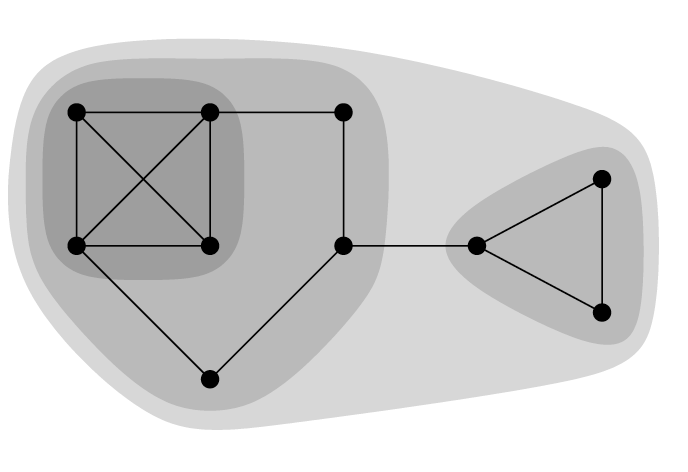
\includegraphics[width=0.55\linewidth]{figure/groups}
\end{figure}
\begin{figure}
    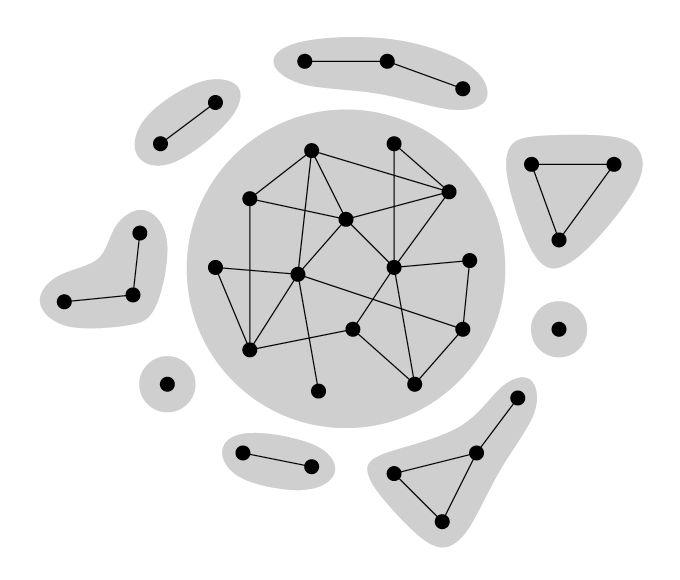
\includegraphics[width=0.55\linewidth]{figure/components}
\end{figure}
\end{column}
\end{columns}

\end{frame}


\begin{frame}
{Network measures}

\begin{columns}
\begin{column}{0.6\textwidth}
  \begin{description}
  \item<1-> [Transitivity of edges] Alice \textit{friend of} Bob \textit{friend of} Cat \textit{friend of} Alice
\item<2-> [Reciprocity of edges] Alice  \textit{friend of} Bob \textit{friend of} Alice
\item<3-> [Similarity of vertices] extent to which the \textit{neighbourhood} of vertices is similar
\item<4-> [Homophily of vertices] tendency to associate with similar vertices
  \end{description}
\end{column}
\begin{column}{0.4\textwidth}
\begin{figure}
    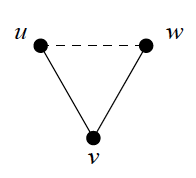
\includegraphics[width=0.35\linewidth]{figure/transitivity.png}
\end{figure}
\begin{figure}
    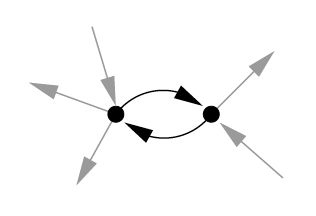
\includegraphics[width=0.4\linewidth]{figure/reciprocity.png}
\end{figure}
\begin{figure}
    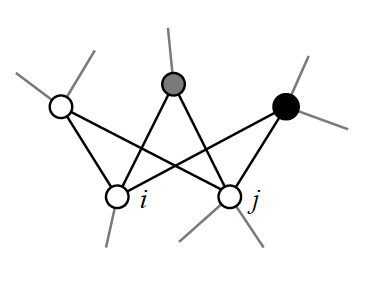
\includegraphics[width=0.4\linewidth]{figure/similarity.png}
\end{figure}
\end{column}
\end{columns}

\end{frame}

\begin{frame}

\begin{figure}
    \centering
    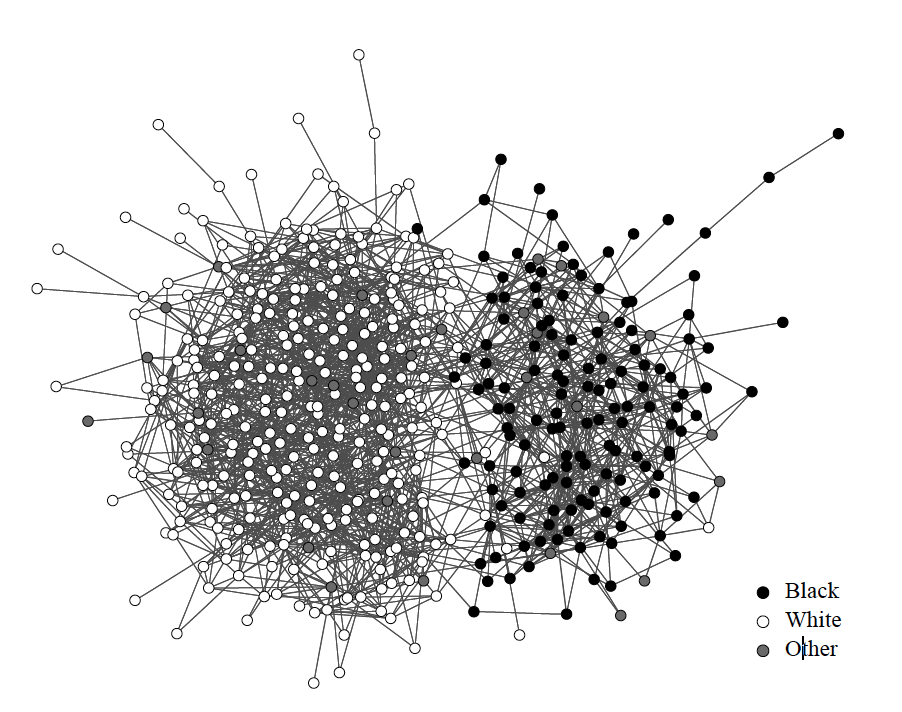
\includegraphics[width=0.55\textwidth]{figure/race_network}
\caption{Friendship network at a US high school \autocite[221]{newman_networks_2010}.}
\end{figure}

\end{frame}

\begin{frame}
{Community detection}

The goal of a community detection algorithm is simply to separate nodes into groups that have only a few edges \textit{between} them and many edges \textit{within}.

\begin{figure}
    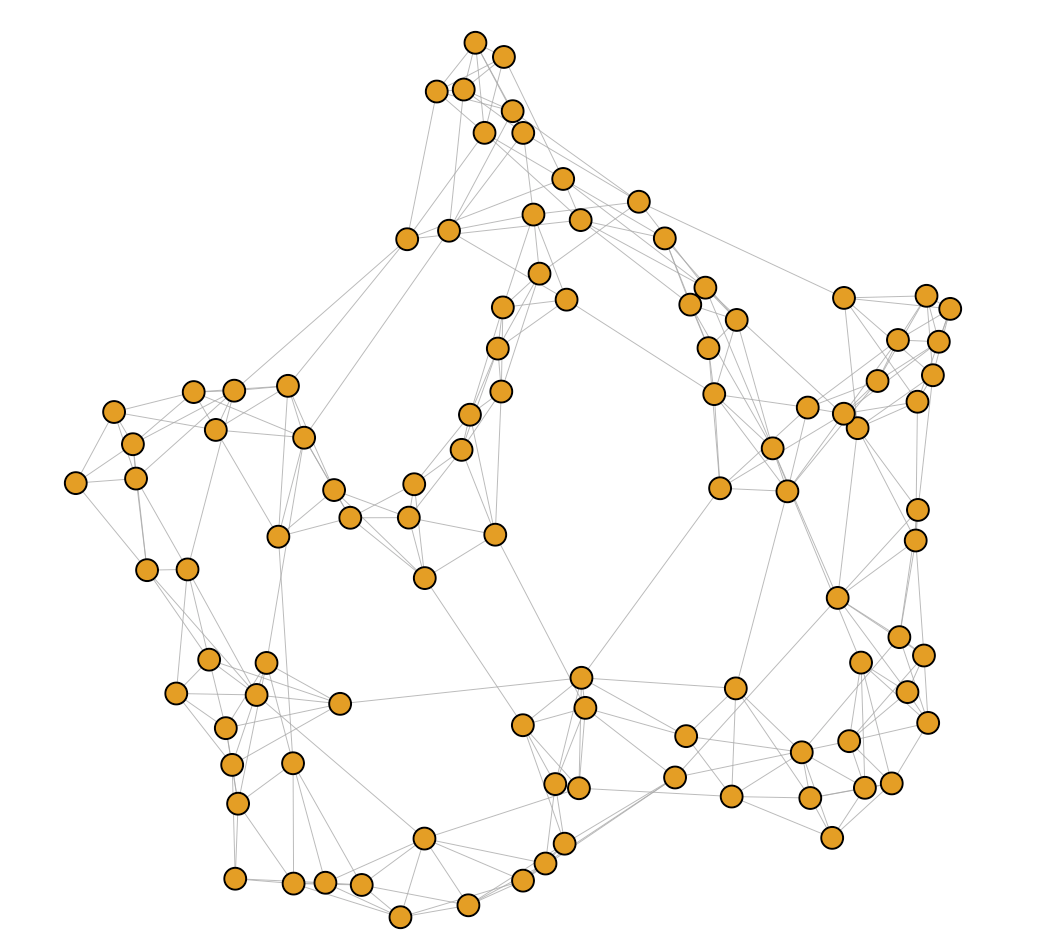
\includegraphics[width=0.4\linewidth]{figure/sample_smallworld}
\caption{A randomly generated network with 100 vertices and 300 edges}
\end{figure}

\end{frame}

\begin{frame}
{Community detection}

How many communities do you see in this network?

\begin{figure}
    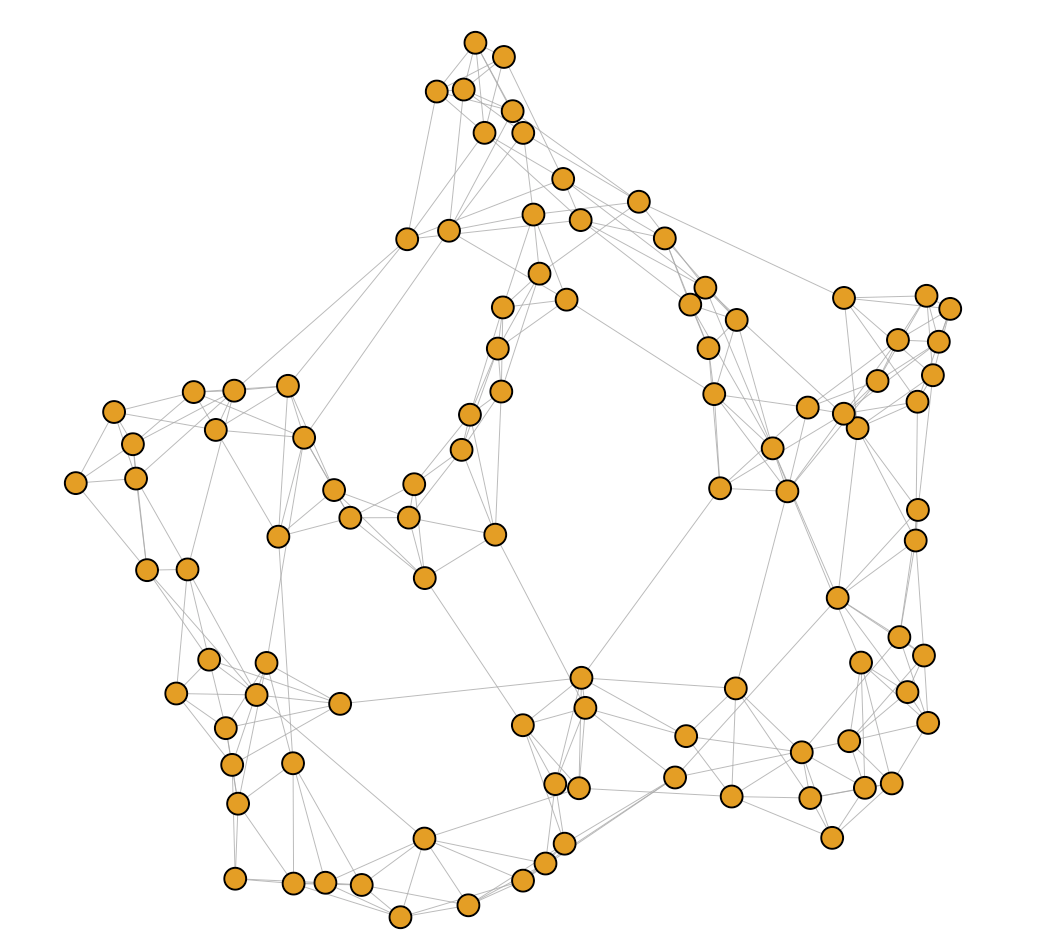
\includegraphics[width=0.4\linewidth]{figure/sample_smallworld}
\end{figure}

\end{frame}

\begin{frame}
{Community detection}

\begin{figure} 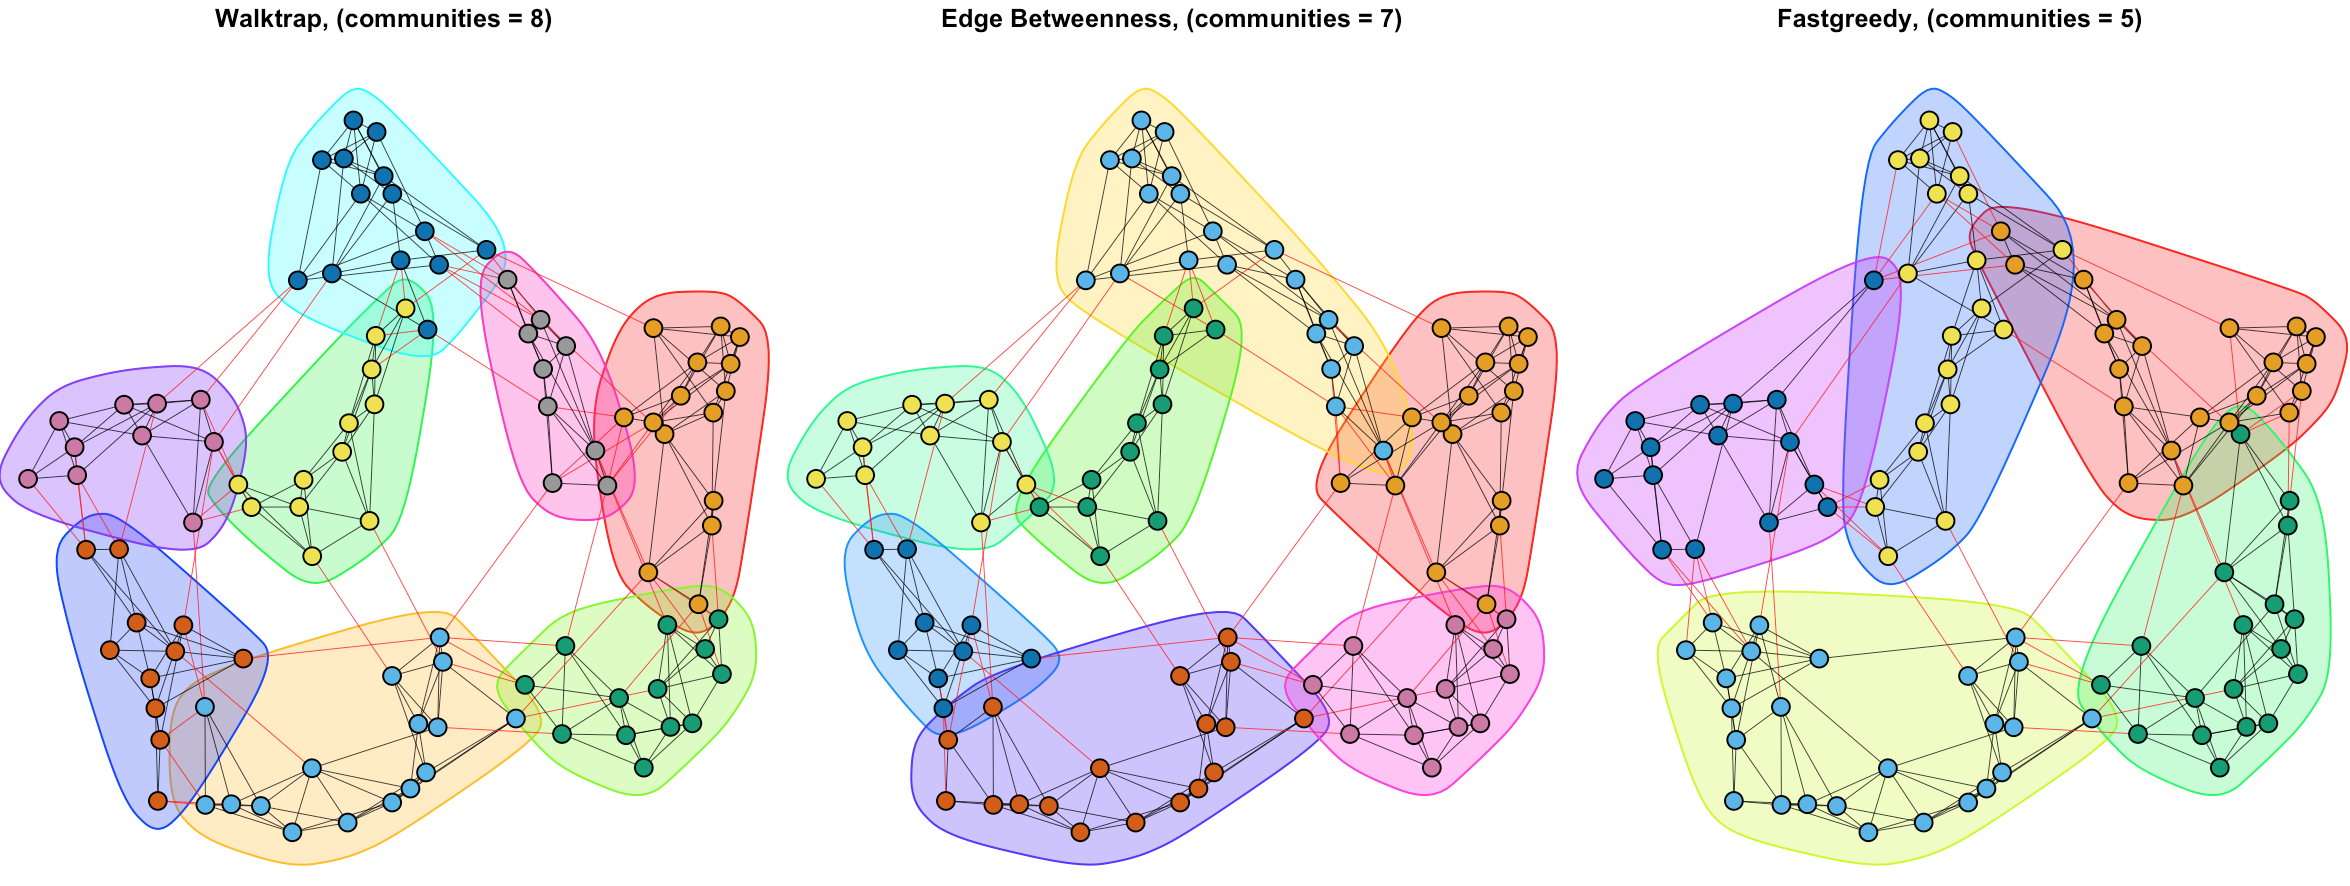
\includegraphics{figure/sample_smallworld_communities}
\end{figure}

\end{frame}


\begin{frame}

\begin{columns}

\begin{column}{0.6\textwidth}
\begin{figure}
    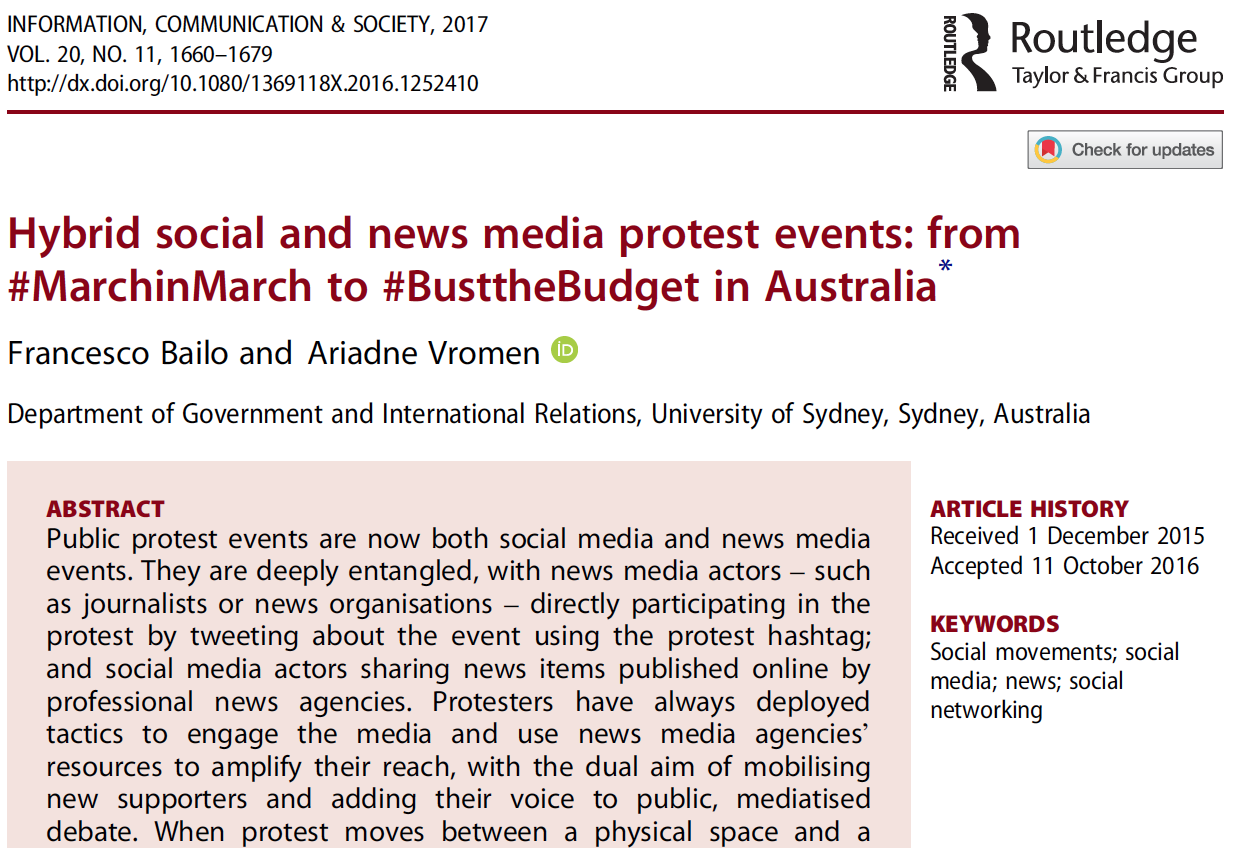
\includegraphics{figure/paper_bailo}
\end{figure}
\end{column}

\begin{column}{0.4\textwidth}
\begin{figure}
    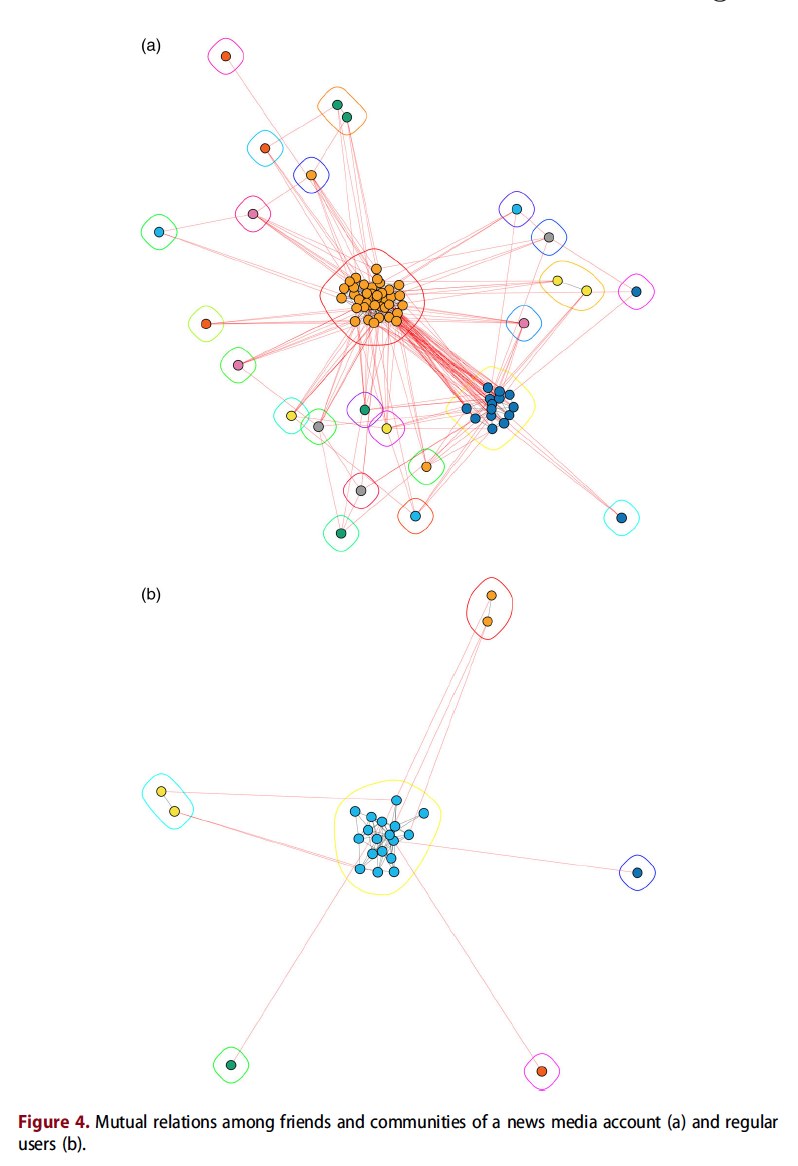
\includegraphics{figure/paper_network}
\end{figure}
\end{column}

\end{columns}

\end{frame}

\subsection{Tools}

\begin{frame}

\centering \textbf{Easy, small n}: Gephi (\url{gephi.org})

\begin{figure}
    \centering
    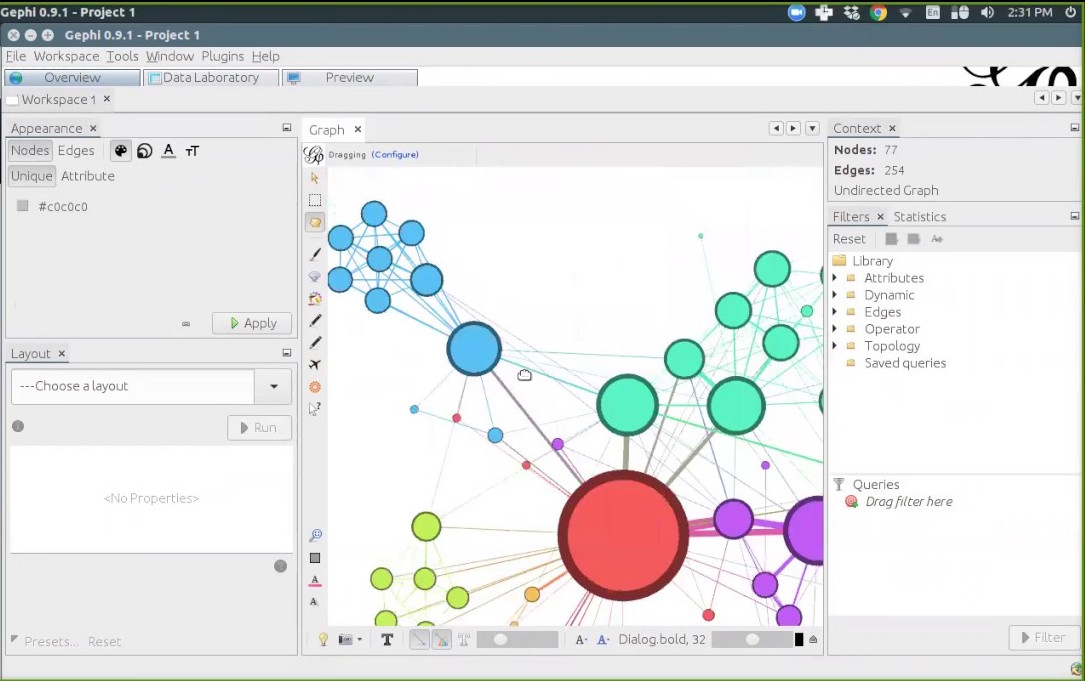
\includegraphics[width=0.65\textwidth]{figure/gephi.jpg}
\end{figure}

\end{frame}

\begin{frame}

\centering \textbf{Hard, big n} igraph package (\url{igraph.org}) in R (\url{www.r-project.org}) or Python (\url{www.python.org})

\begin{figure}
    \centering
    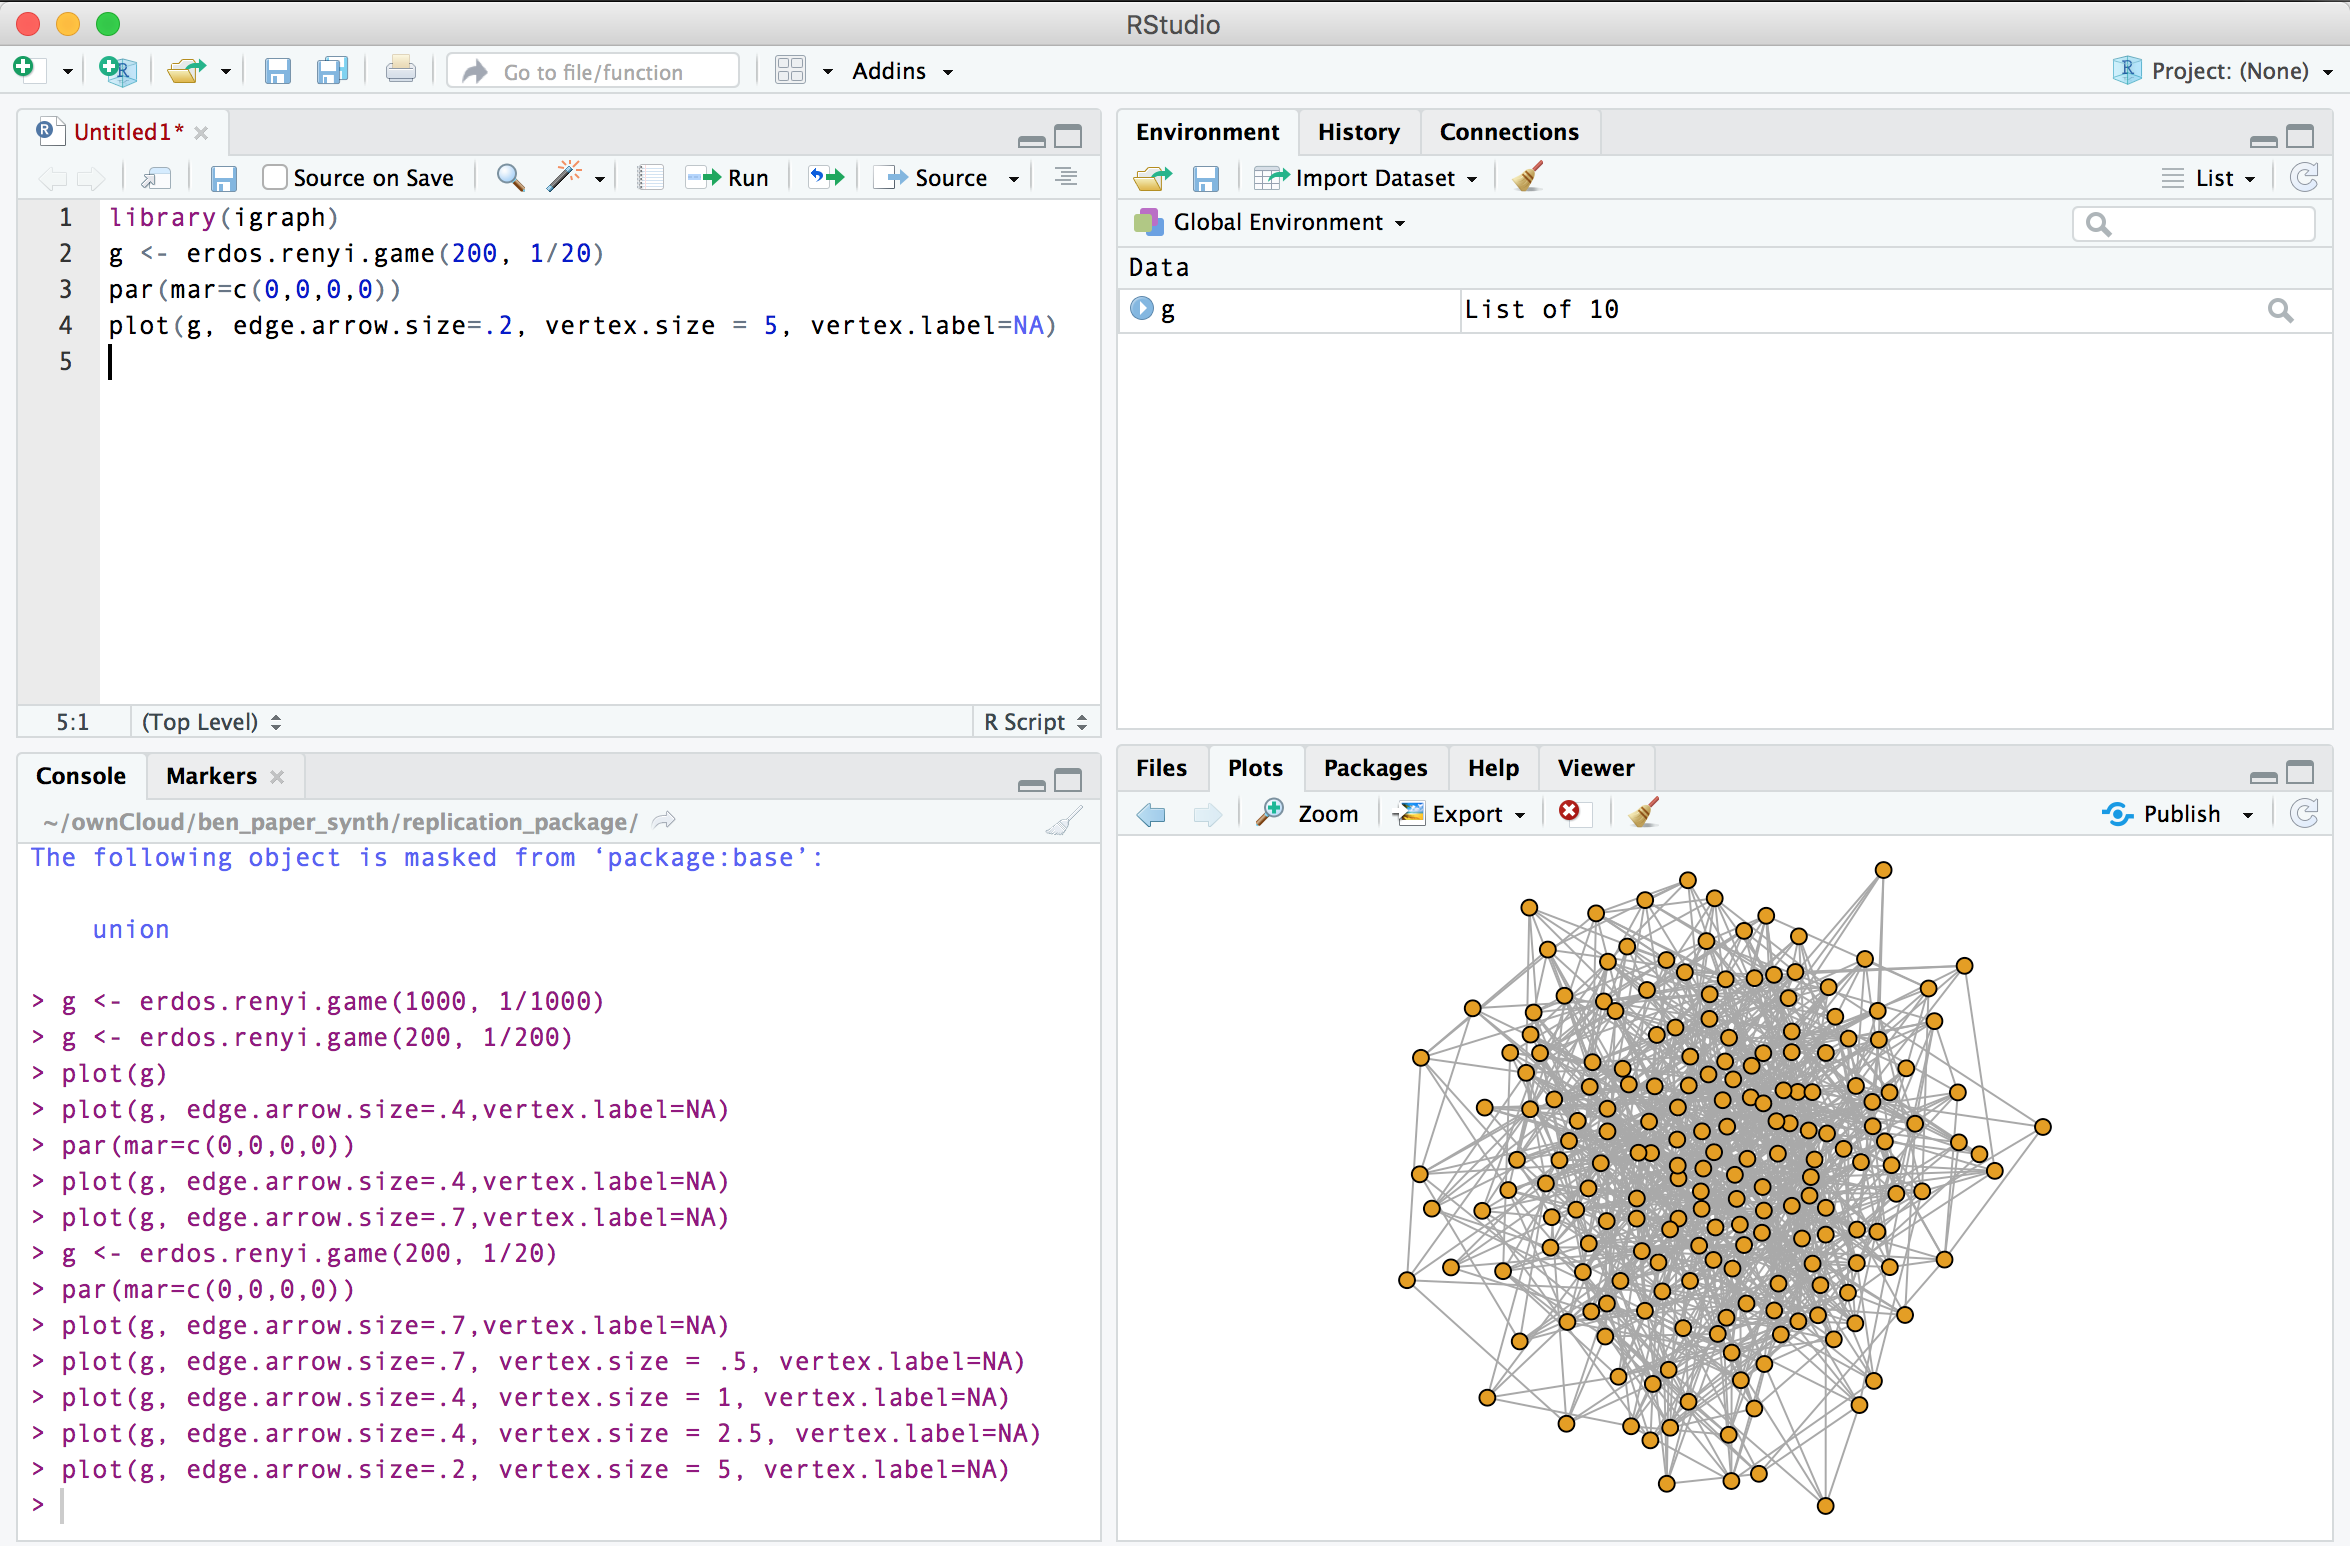
\includegraphics[width=0.6\textwidth]{figure/igraph}
\end{figure}

\end{frame}

\subsection{Resources}

\begin{frame}

Getting started bibliography:

\begin{description}
\item [Easy] \customcite{scott_what_2012}
\item [Important] \customcite{marin_social_2011}
\item [Hard] \customcite{newman_networks_2010}
\end{description}

\end{frame}


\begin{frame}

Tutorials for beginners by Katherine Ognyanova (Rutgers University):

\begin{figure}
    \centering
    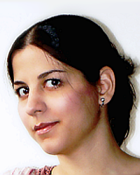
\includegraphics[width=0.1\textwidth]{figure/Ognyanova_Katherine}
\end{figure}


\begin{itemize}
\item Network visualisation with Gephi (\url{kateto.net/sunbelt2016})
\item Network visualization with R (\url{kateto.net/network-visualization})
\item Network Analysis and Visualization with R and igraph (\url{kateto.net/networks-r-igraph})
\end{itemize}

\end{frame}

\section{Text analysis}

\subsection{Another very short introduction}

\begin{frame}

Quantitative text analysis is necessary when the manual coding of documents is not feasible or acceptable. 

When you face a large \textbf{corpus} of \textbf{documents}, you might want some methods to automatically:

\begin{enumerate}

\item Find patterns within the documents,

\item Compare (and maybe group) documents.

\end{enumerate}

\end{frame}

\begin{frame}[fragile]
\frametitle{Finding patterns}

A textual pattern is as simple as \texttt{dog}.

\begin{itemize}

\item Finding patterns doesn't involve any statistical analysis.

\item But you might need to use regular expressions (a.k.a. \enquote{regex}) if your pattern is complex.

\end{itemize}

\end{frame}

\begin{frame}[fragile]
\frametitle{Finding patterns}

Let's say that you want to find in your corpus all the instances of \texttt{dog} and \texttt{cat}.

\begin{description}

\item<1->[You want to find] \enquote{I have two \underline{dog}s and a \underline{cat}} or \enquote{\underline{Cat}s are felines}

\item<2->[But you don't want to find]  \enquote{the \underline{cat}egorization of syntactic \underline{cat}egories}

\item<3-> You need a regular expression like: {\LARGE\verb=\b(cats?|dogs?)\b=} 

\end{description}

{\tiny (\href{https://regexr.com/3oqld}{link to interactive example})}

\end{frame}

\begin{frame}[fragile]
\frametitle{Finding patterns}

A few simple regex topics:

\begin{description}

\item<1->[Quantifier] \bverb|?|

\begin{itemize}

\item<2-> \bverb|abc?| matches a string that has \enquote{ab} followed by zero or one \enquote{c}

\end{itemize}

\item<3->[OR operator] \bverb=|=

\begin{itemize}

\item<4-> \bverb=a(b|c)= matches a string that has \enquote{a} followed by \enquote{b} or \enquote{c}

\end{itemize}

\item<5->[Boundaries]\bverb|\b|

\begin{itemize}

\item<6-> \bverb=\babc\b= matches only a whole word

\end{itemize}

\end{description}

{\footnotesize Exercise: Go to \texttt{\href{https://regexr.com/3os9b}{regexr.com/3os9b}} (not with Explorer) and enter a regular expression to match \enquote{France} but also \enquote{French}}.

\end{frame}

\begin{frame}
\frametitle{Comparing documents}

Comparing documents involves statistical analysis and matrix algebra (while finding patterns doesn't). It usually relies on Natural-language processing (NLP), the branch of computer science that studies the human language and its interactions with the machines. 

In its most primordial application, NLP treats documents as \textbf{bag-of-words} (BoW):
\begin{itemize}
\item  The \textit{position} of terms within the document is disregarded,
\item What counts is the \textit{frequency} of the terms.
\end{itemize}

\end{frame}

\begin{frame}
\frametitle{Comparing documents}

Let's see how we process documents in a common NLP application.

\begin{itemize}

\item<1-> We remove from the documents all the stop-words;

\item<2-> doc1 = "drugs hospitals doctors" \\
doc2 = "smog pollution environment" \\
doc3 = "doctors hospitals healthcare" \\
doc4 = "pollution environment water" \\

\item<3-> We count the frequency of each term in each document, and we produce a term-document matrix

\end{itemize}

\end{frame}

\begin{frame}
\frametitle{Comparing documents}

\begin{table}[ht]
\centering
\begin{tabular}{rrrrr}
  \hline
 & doc1 & doc2 & doc3 & doc4 \\ 
  \hline
doctor & 1 & 0 & 1 & 0 \\ 
  drug & 1 & 0 & 0 & 0 \\ 
  environ & 0 & 1 & 0 & 1 \\ 
  healthcar & 0 & 0 & 1 & 0 \\ 
  hospit & 1 & 0 & 1 & 0 \\ 
  pollut & 0 & 1 & 0 & 1 \\ 
  smog & 0 & 1 & 0 & 0 \\ 
  water & 0 & 0 & 0 & 1 \\ 
   \hline
\end{tabular}
\caption{Term-document matrix. Terms were stemmed.} 
\label{tab:example1-tf-table}
\end{table}

\end{frame}


\begin{frame}
\frametitle{Bag of Words (BoW)}
\begin{itemize}
    \item \textbf{Concept:} Text representation as a bag of its words, ignoring the order.
    \item \textbf{Representation:} Fixed-length vectors, counting word occurrences or indicating presence/absence.
    \item \textbf{Advantages:} Simple, good for specific tasks like spam detection.
    \item \textbf{Limitations:} Ignores context and semantics, leading to sparse, high-dimensional vectors.
\end{itemize}
\end{frame}

\begin{frame}
\frametitle{Embeddings (used by the Large Language Models)}
\begin{itemize}
    \item \textbf{Concept:} Dense, low-dimensional vectors representing words, capturing semantic meanings.
    \item \textbf{Representation:} Continuous vectors that reflect context and relationships between words.
    \item \textbf{Advantages:} Captures semantics, reduces dimensionality and is versatile for various NLP tasks.
    \item \textbf{Limitations:} Requires more computational resources, less intuitive.
\end{itemize}
\end{frame}

\subsection{Tools}

\begin{frame}

\begin{itemize}

\item Nvivo (\url{www.qsrinternational.com/nvivo})

\item Regular Expression (\url{regexr.com})

\item R (\url{www.r-project.org}) or Python (\url{www.python.org})

\item ChatGPT and other Large Language Models... 

\end{itemize}

\end{frame}

\begin{frame}

\end{frame}

\subsection{Resources}

\begin{frame}

\begin{description}

\item [Introductory] \customcite{jockers_text_2014}

\item [Introductory] \customcite{bird_natural_2009}

\item [Hard] \customcite{manning_introduction_2008}

\end{description}

\end{frame}

\section{Ethics}

\begin{frame}
{Issues with relational data}

\begin{columns}

\begin{column}{0.4\textwidth}
\begin{figure}
    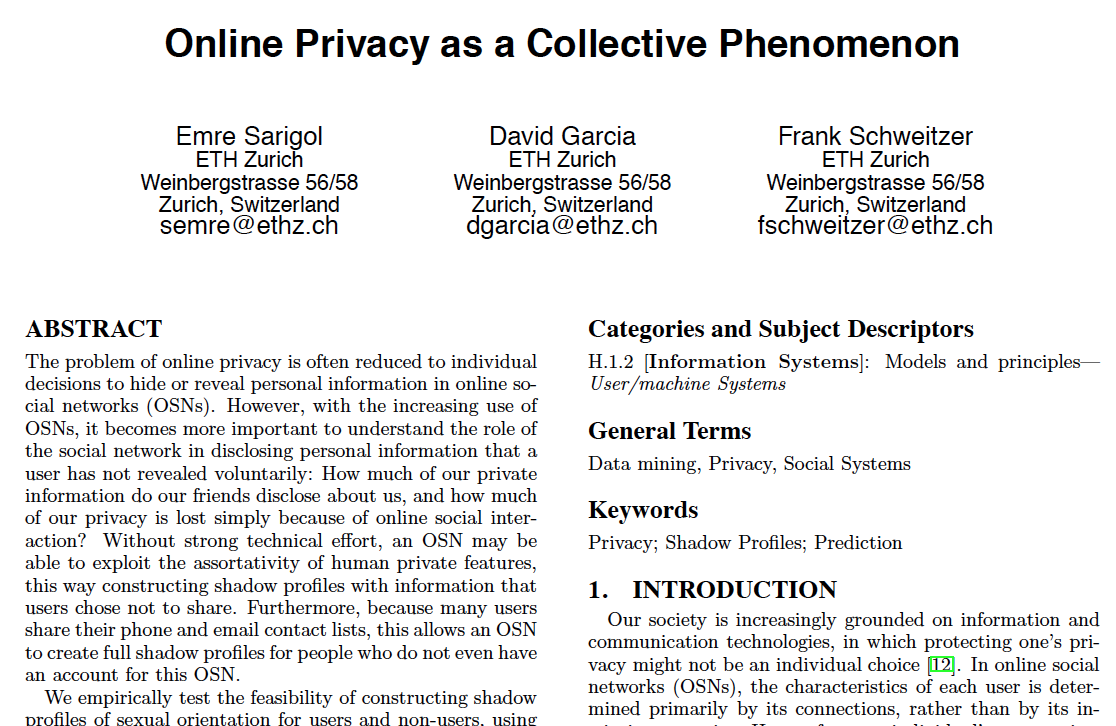
\includegraphics[width=1\textwidth]{figure/garcia_paper}
\caption{\customcite{sarigol_online_2014}}
\end{figure}
\end{column}

\begin{column}{0.25\textwidth}
\begin{figure}
    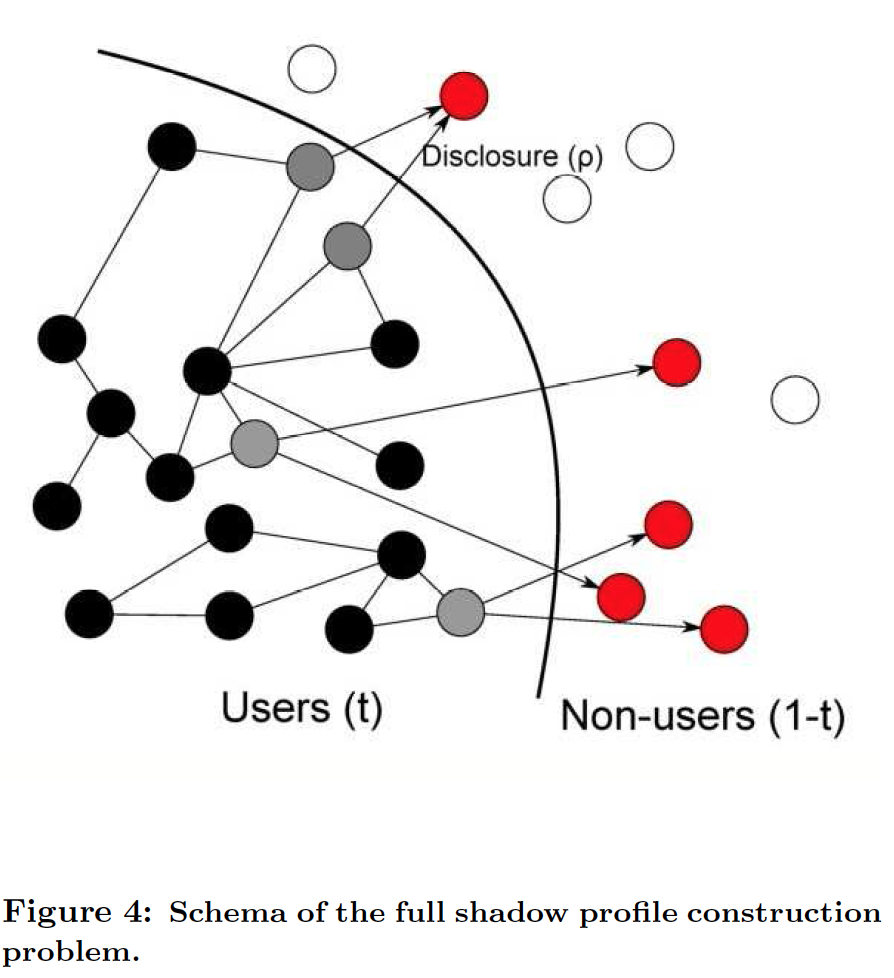
\includegraphics[width=1\textwidth]{figure/garcia_fig1}
\end{figure}
\end{column}

\begin{column}{0.35\textwidth}
\begin{figure}
    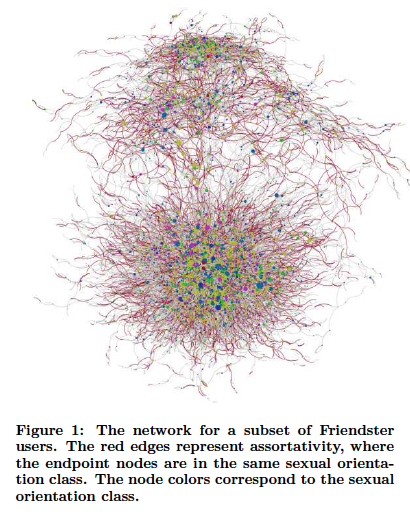
\includegraphics[width=1\textwidth]{figure/garcia_fig2}
\end{figure}
\end{column}
\end{columns}

\end{frame}

\begin{frame}
{Ethics in the digital age: Open issues}

\begin{itemize}

\item Public and Private space. What about online fora (e.g. Facebook public pages?)

\item Informed consent.

\item Right to privacy. But who owns the data?

\end{itemize}

\end{frame}

\nocite{salganik_bit_2018}
\nocite{bailo_hybrid_2017}

\section{My research on social media}

\begin{frame}

\begin{itemize}
\item \fullcite{kongSlippingExtremeMixed2022}
\item  \fullcite{bailoRidingInformationCrises2024}
\item \fullcite{johnsLabellingShadowBans2024}
\end{itemize}

\end{frame}

% Slide 1: Summary Slide

\begin{frame}{Slipping to the extreme}
\item \fullcite{kongSlippingExtremeMixed2022}
\begin{itemize}
  \item This study addresses the infiltration of extreme opinions in online discussions, leveraging machine learning algorithms alongside qualitative research methods.
  \item Aims to bridge the gap between depth of qualitative insights and breadth of quantitative analysis in understanding problematic online speech.
\end{itemize}
\end{frame}

\begin{frame}{Methodology}
\begin{itemize}
  \item Initial qualitative study constructs an ontology of problematic speech, identifying key themes and opinions in social media posts.
  \item Large-scale data collection from Facebook, Twitter, and YouTube, followed by iterative dataset augmentation using a human-in-the-loop approach.
  \item Machine learning models classify and augment the dataset, expanding the initial qualitative study's findings.
\end{itemize}
\end{frame}

\begin{frame}

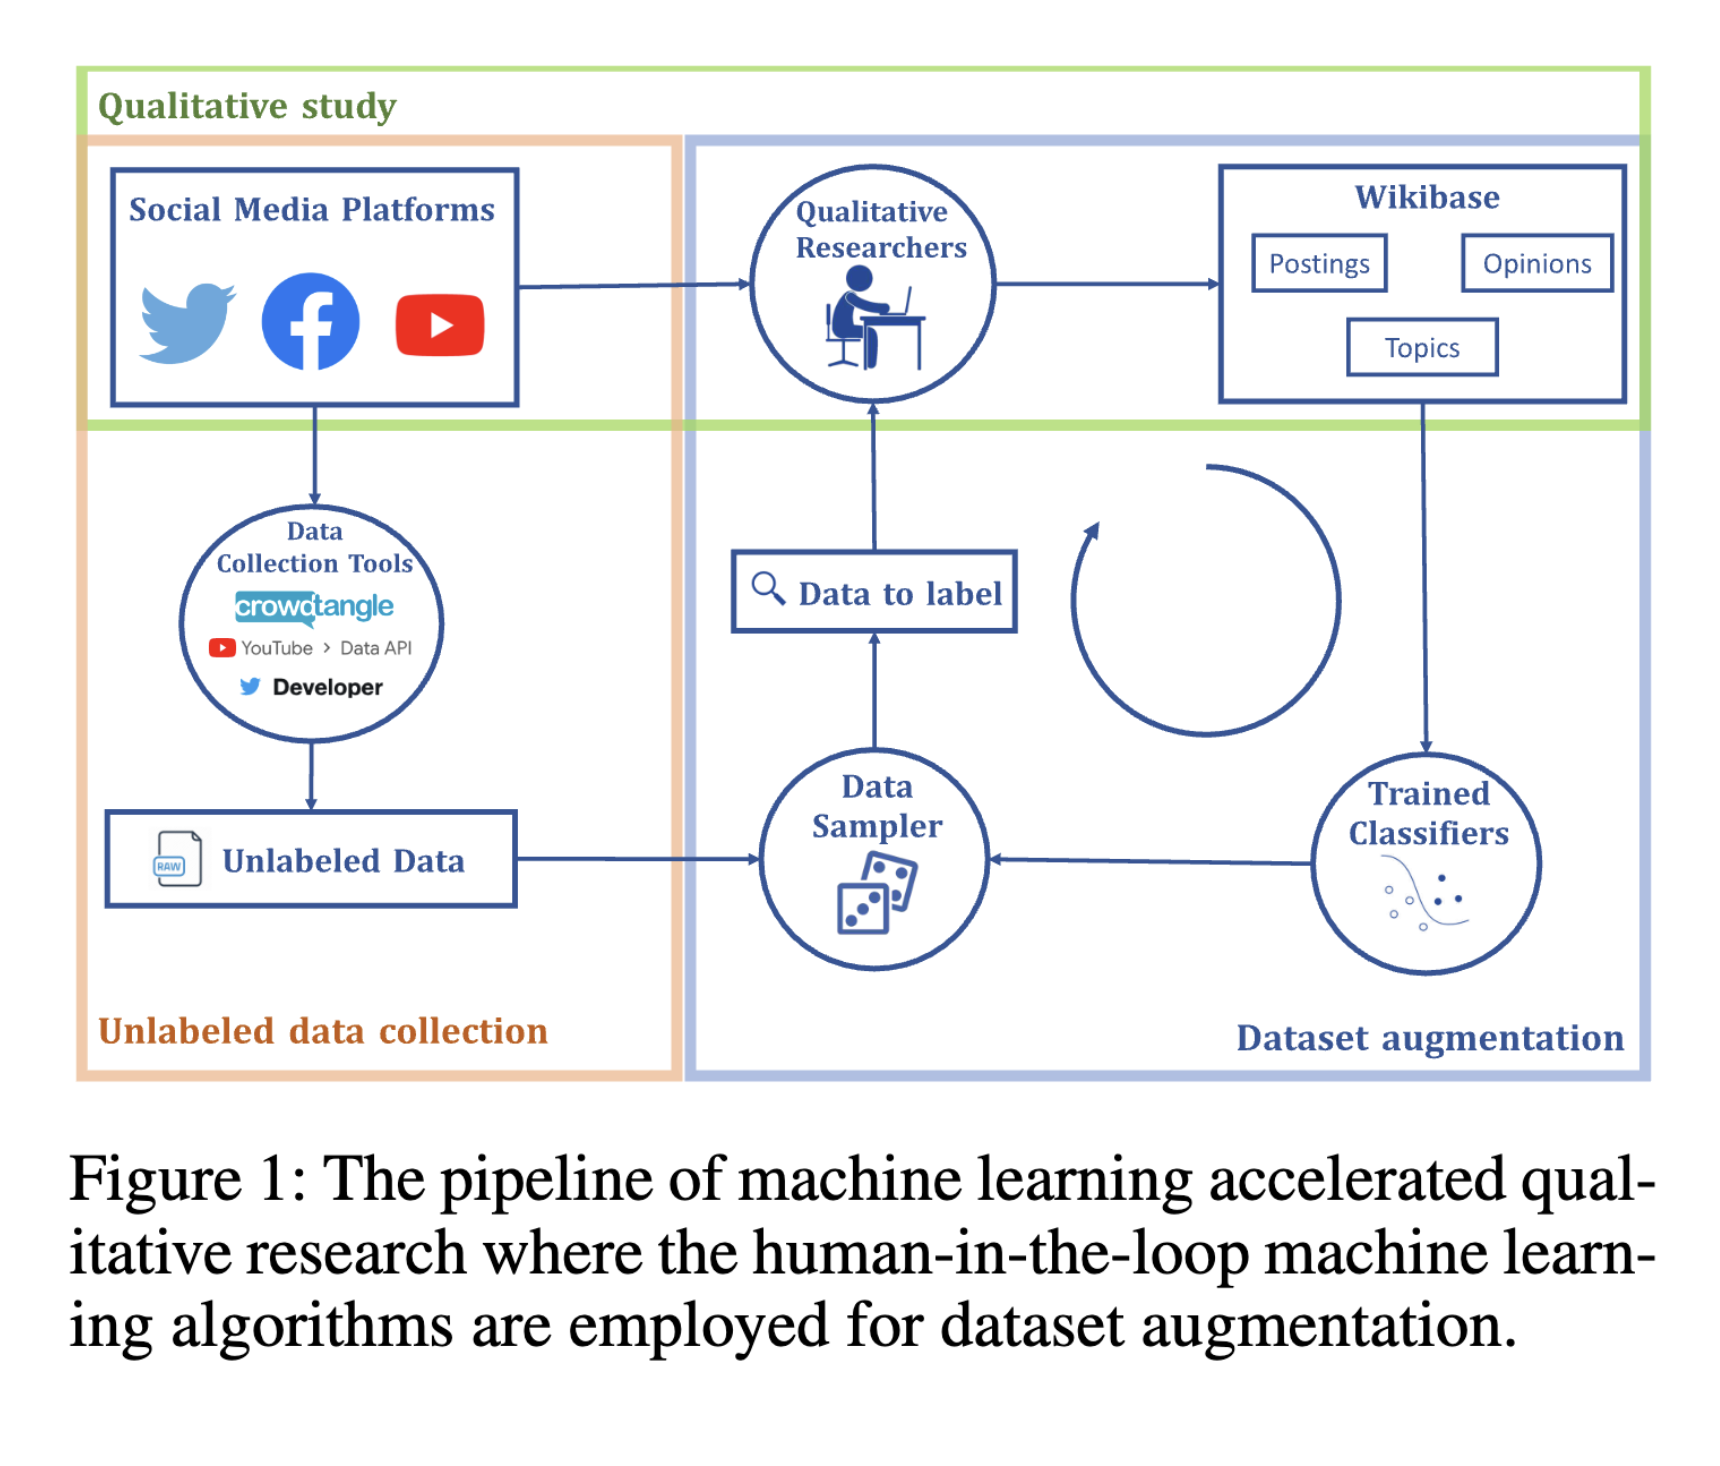
\includegraphics[]{introduction_2h/figure/kongSlippingExtremeMixed2022-fig1.png}

\end{frame}

\begin{frame}{Findings}
\begin{itemize}
  \item The mixed-method approach successfully identifies and expands the dataset, revealing detailed case studies of problematic speech dynamics in specific online communities.
  \item Analysis of opinion emergence and co-occurrence suggests pathways through which extreme opinions enter mainstream online discourse.
\end{itemize}
\end{frame}

% Overview Slide
\begin{frame}
\frametitle{Labelling, shadow bans and community resistance}
\fullcite{johnsLabellingShadowBans2024}
\begin{itemize}
    \item Focus on the effectiveness of Meta's content moderation on Facebook during COVID-19.
    \item Analysis of 18 Australian right-wing/anti-vaccination pages between January 2019 and July 2021.
    \item Integration of engagement metrics, time series analysis, and content analysis.
\end{itemize}
\end{frame}

% Sampling Slide
\begin{frame}
\frametitle{Sampling}
\begin{itemize}
    \item Utilised CrowdTangle to collect data from 21 identified Australian Facebook public accounts.
    \item Final analysis included 18 accounts after excluding those with less than 1\% of relevant posts.
    \item A total of 34,202 postings were analysed.
\end{itemize}
\end{frame}

% Data Analysis Slide
\begin{frame}
\frametitle{Data Analysis}
\begin{itemize}
    \item Performance analysis via CrowdTangle's 'overperforming score' and average number of shares-per-post.
    \item Content and thematic analysis on comments from two overperforming public pages.
    \item Latent Dirichlet Allocation (LDA) for topic modelling and exploration.
\end{itemize}
\end{frame}

\begin{frame}

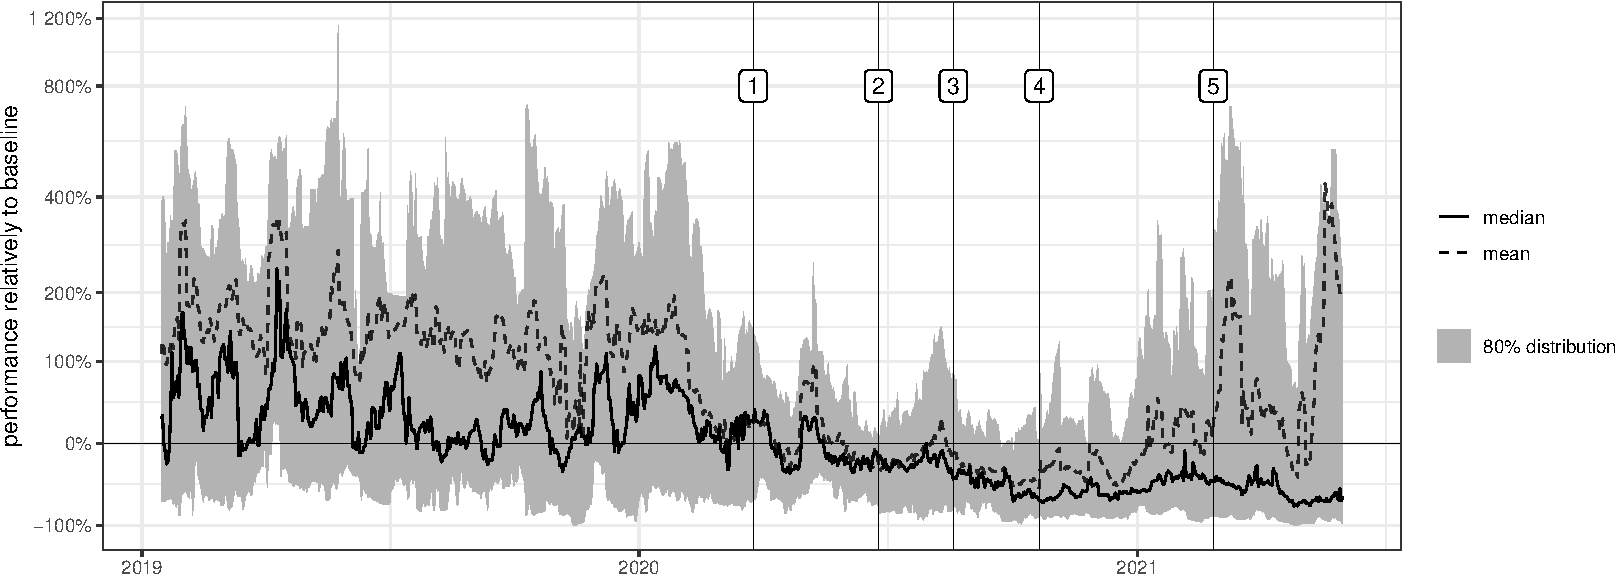
\includegraphics[]{introduction_2h/figure/figure4-1.pdf}

\end{frame}

% Policy Review Slide
\begin{frame}
\frametitle{Policy Review}
\begin{itemize}
    \item Examination of Meta's content moderation and recommendation policy announcements.
    \item Focus on policies introduced from January 2020 to July 2021 relevant to Facebook.
    \item Analysis juxtaposed against key policy announcements and page performance.
\end{itemize}
\end{frame}

% Findings Slide
\begin{frame}
\frametitle{Key Findings}
\begin{itemize}
    \item Meta's content moderation systems showed partial effectiveness.
    \item Identified trends in content labelling and 'shadow banning' resistance by communities.
    \item Highlighted the importance and challenges of transparent and consistent moderation policies.
\end{itemize}
\end{frame}


\section{Bonus: Spatial analysis}

\begin{frame}
{Spatial analysis}
\begin{columns}
\begin{column}{0.7\textwidth}
\begin{figure}
    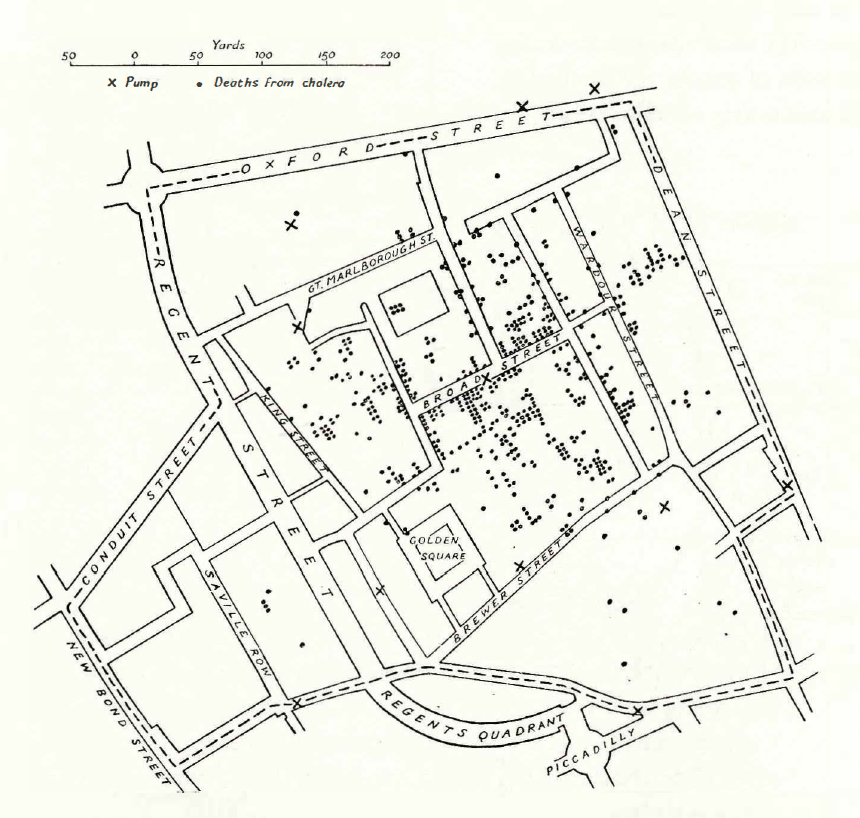
\includegraphics[width=0.9\textwidth]{figure/john_snow_map}
\end{figure}
\end{column}
\begin{column}{0.3\textwidth}
Redrawing of John Snow's map of cases of cholera during the London outbreak of 1854 \autocite[24]{tufte_visual_2001}
\end{column}
\end{columns}
\end{frame}

\begin{frame}
{Tool for spatial analysis}

\begin{itemize}

\item QGIS (\url{qgis.org})

\end{itemize}

\begin{figure}
    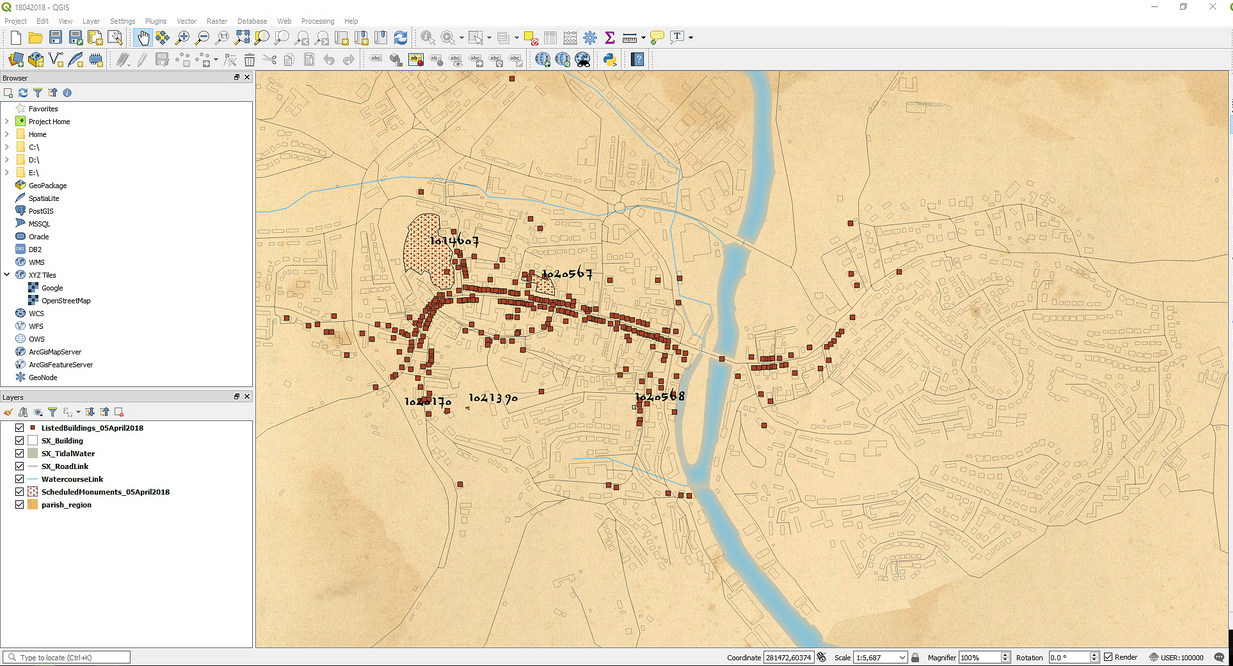
\includegraphics[width=0.8\textwidth]{figure/qgis}
\end{figure}

\end{frame}


\begin{frame}[allowframebreaks]
\printbibliography
\end{frame}



\end{document}
%%% Local Variables:
%%% mode: latex
%%% TeX-master: t
%%% End:
